\documentclass[8pt]{beamer}\usepackage[]{graphicx}\usepackage[]{color}

%\setbeamercovered{transparent}

\usefonttheme{professionalfonts} % using non standard fonts for beamer
\usefonttheme{serif} % default family is serif
\usepackage{fontspec}
\setmainfont{Liberation Serif}

\documentclass{article}
\usepackage{fancyhdr}


\pagestyle{fancy}
\fancyhf{}
\rhead{Ryan Giordano}
\lhead{Research Statement}
\rfoot{Page \thepage}

\usepackage{tabularx}

% \usepackage{fancyhdr}
% \pagestyle{fancy}

% \fancyfoot{}
% \fancyfoot[C]{Rough draft---do not distribute}

\usepackage{etoolbox}


\usepackage{microtype}
\usepackage{graphicx}
\usepackage{subfigure}
\usepackage{booktabs} % for professional tables
\usepackage{xcolor}
\usepackage[hidelinks=True]{hyperref}
\usepackage{xargs}[2008/03/08]

% Documentation
% http://ftp.math.purdue.edu/mirrors/ctan.org/macros/latex/contrib/refstyle/refstyle.pdf
\usepackage{refstyle}
\usepackage{varioref} % Use refstyle instead of varioref directly.

\usepackage{amsmath}
\usepackage{amssymb}
\usepackage{amsfonts}
\usepackage{amsthm}
\usepackage{mathrsfs} % For mathscr
\usepackage{mathtools}

\usepackage[authoryear]{natbib}
\bibliographystyle{apalike}

\usepackage{geometry}
\geometry{margin=1.5in}

% % This file contains the boilerplate that knitr would put at the top of
% a knitr document if you ran knitr with \begin{document} ... \end{document}.
% By including it once in the main document, you can knit and \input{}
% Rnw files that contain only individual sections.

\usepackage[]{graphicx}
\usepackage[]{color}
%% maxwidth is the original width if it is less than linewidth
%% otherwise use linewidth (to make sure the graphics do not exceed the margin)
\makeatletter
\def\maxwidth{ %
  \ifdim\Gin@nat@width>\linewidth
    \linewidth
  \else
    \Gin@nat@width
  \fi
}
\makeatother

\definecolor{fgcolor}{rgb}{0.345, 0.345, 0.345}
\newcommand{\hlnum}[1]{\textcolor[rgb]{0.686,0.059,0.569}{#1}}%
\newcommand{\hlstr}[1]{\textcolor[rgb]{0.192,0.494,0.8}{#1}}%
\newcommand{\hlcom}[1]{\textcolor[rgb]{0.678,0.584,0.686}{\textit{#1}}}%
\newcommand{\hlopt}[1]{\textcolor[rgb]{0,0,0}{#1}}%
\newcommand{\hlstd}[1]{\textcolor[rgb]{0.345,0.345,0.345}{#1}}%
\newcommand{\hlkwa}[1]{\textcolor[rgb]{0.161,0.373,0.58}{\textbf{#1}}}%
\newcommand{\hlkwb}[1]{\textcolor[rgb]{0.69,0.353,0.396}{#1}}%
\newcommand{\hlkwc}[1]{\textcolor[rgb]{0.333,0.667,0.333}{#1}}%
\newcommand{\hlkwd}[1]{\textcolor[rgb]{0.737,0.353,0.396}{\textbf{#1}}}%
\let\hlipl\hlkwb

\usepackage{framed}
\makeatletter
\newenvironment{kframe}{%
 \def\at@end@of@kframe{}%
 \ifinner\ifhmode%
  \def\at@end@of@kframe{\end{minipage}}%
  \begin{minipage}{\columnwidth}%
 \fi\fi%
 \def\FrameCommand##1{\hskip\@totalleftmargin \hskip-\fboxsep
 \colorbox{shadecolor}{##1}\hskip-\fboxsep
     % There is no \\@totalrightmargin, so:
     \hskip-\linewidth \hskip-\@totalleftmargin \hskip\columnwidth}%
 \MakeFramed {\advance\hsize-\width
   \@totalleftmargin\z@ \linewidth\hsize
   \@setminipage}}%
 {\par\unskip\endMakeFramed%
 \at@end@of@kframe}
\makeatother

\definecolor{shadecolor}{rgb}{.97, .97, .97}
\definecolor{messagecolor}{rgb}{0, 0, 0}
\definecolor{warningcolor}{rgb}{1, 0, 1}
\definecolor{errorcolor}{rgb}{1, 0, 0}
\newenvironment{knitrout}{}{} % an empty environment to be redefined in TeX

\usepackage{alltt}



\def\argmax#1{\mathrm{argmax}_{#1}\,}
\def\argmin#1{\mathrm{argmin}_{#1}\,}
\def\cov#1#2{\mathrm{Cov}_{#1}\left( #2\right)\,}
\def\expect#1#2{\mathbb{E}_{#1}\left[ #2\right]\,}
\def\var#1#2{\mathrm{Var}_{#1}\left( #2\right)\,}
\def\cumulant#1#2{\mathcal{K}_{#1}\left( #2\right)\,}
\def\expecthat#1#2{\hat{\mathbb{E}}_{#1}\left[ #2\right]\,}
\newcommand{\fracat}[3]{\left. \frac{#1}{#2} \right|_{#3}}
\newcommand{\norm}[1]{\left\Vert#1\right\Vert}
\newcommand{\abs}[1]{\left|#1\right|}
\def\diag#1{\textrm{Diag}\left( #1\right)}
\def\ord#1{\mathcal{O}\left( #1\right)}
\def\ordp#1{\mathcal{O}_p\left( #1\right)}
\def\gauss#1{\mathcal{N}\left( #1\right)}
\def\trans{\intercal} % transpose
\def\id{I} % Identity matrix
\def\iid{\overset{iid}{\sim}}
\def\rdom#1{\mathbb{R}^{#1}}
\def\ind#1{\mathbb{I}\left(#1\right)}
\def\varemp#1{\hat{\mathrm{Var}}\left(#1\right)}


% Sets of data in the survey and target

\def\tarcol#1{\textcolor{red}{#1}}
\def\surcol#1{\textcolor{blue}{#1}}


\def\sur{\mathcal{S}}
\def\tar{\mathcal{T}}
\def\nsur{{\surcol{N_S}}}
\def\ntar{{\tarcol{N_T}}}

\def\Nsur{{\surcol{N_S}}}
\def\Ntar{{\tarcol{N_T}}}


\def\postsur{\surcol{\p(\theta \vert \textrm{Survey data})}}
\def\post{\postsur}

\def\f{f}
\def\sumn{\sum_{n=1}^N}
\def\meann{\frac{1}{N} \sum_{n=1}^N}
\def\sumsur{\sum_{i=1}^\Nsur}
\def\sumtar{\sum_{j=1}^\Ntar}
\def\meansur{\frac{1}{\Nsur} \sumsur}
\def\meantar{\frac{1}{\Ntar} \sumtar}


% Distributions of x or (x, y) in the survey and target
% p is common to both (for p(y | x))
\def\psur{\surcol{{\mathcal{P}_{S}}}}
\def\ptar{\tarcol{\mathcal{P}_{T}}}
%\def\ptarhat{{\hat{\mathcal{P}}_{T}}}
\def\p{\mathcal{P}}
%\def\post{\p(\beta \vert \sur )}
\newcommand{\postd}[1][\delta]{\p(\beta \vert \sur, #1)}



% Different MrP estimates
\def\mrp{\mathrm{MrP}}
\def\ols{\mathrm{OLS}}
\def\cal{\mathrm{WGT}}
\def\glm{\mathrm{GLM}}
\def\hwt{\mathrm{HT}} % Horwitz--Thompson

% Population estimator
\newcommand{\muhat}[1][]{\hat{\mu}^{#1}}
\newcommand{\w}[1][]{w^{#1}}

\newcommand{\muhatmrp}[1][\Ysur]{\tarcol{\muhat[\mrp]}(\surcol{#1})}
\newcommand{\muhatcw}[1][\Ysur]{\tarcol{\muhat[\cal]}(\surcol{#1})}


% Link function, usually expit.
\def\m{m}
\def\mhat{\hat{\m}}
\def\minv{\m^{-1}}
\def\betahat{\hat{\beta}} % Regression coefficient
\def\betastar{\overset{*}{\beta}} % Regression coefficient
\def\betadom{\rdom{D_\beta}}
% \def\thetahat{\hat{\theta}} % All parameters
% \def\thetastar{\overset{*}{\theta}} % All parameters

% BCLT quantities
\def\g{g} % Quantity of interest
\def\info{\mathcal{I}}
\def\infohat{\hat{\info}}
\def\resid{\mathcal{E}}
\def\V{V} % Limiting variance
\def\Vhat{\hat{V}} % Limiting variance estimate

\def\tautil{\tilde{\tau}} % Intermediate value for covariate balance
\def\A{A} % Log partition function
\def\Ap{A^{+}} % Log partition function
\def\Agrad#1{A_{(#1)}} % Log partition function derivative
\def\betaball{\mathcal{B}_{\delta}} % Neighborhood of thetastar
\def\deltamax{\delta_{+}} % Maximum value of \delta
\def\deltadom{[0, \deltamax]} % Maximum value of \delta

% % Estimating equation
% \def\G{G}
% \def\H{H}
% \def\Hhat{\hat{H}}
% \def\t{t} % Implicit function theorem perturbation


% Different "weights"


\def\thetahat{\hat{\theta}}

% The regressors actually used in MrP (as opposed to x)
% which is all observed data.
\def\Ztar{Z_{\tar}}
\def\Zsur{Z_{\sur}}
\def\z{z}

% THe full observed regressors, possibly distinct from what 
% is actually in the regression
\def\x{\mathbf{x}}
\def\X{X}
\def\Xtar{X_{\tar}}
\def\Xsur{X_{\sur}}


% The response weighting error
\def\r{r}  % New (missing) regressor
\def\rdim{D_r}  % New (missing) regressor
\def\Rsur{R_{\sur}}  % New (missing) sample regressor
\def\Rtar{R_{\tar}}  % New (missing) target regressor

% % dyhat / dy
% \def\W{W}
\def\w{w}
\def\wmrp{w^{\mrp}}
\def\wv{\mathbf{w}}
% \def\Wols{W_{OLS}}
% \def\Wglm{W_{GLM}}
% \def\Wbhm{W_{BHM}}


% The response vector and values
\def\y{y}
\def\yhat{\hat{y}}
\def\ytil{\tilde{y}}
\def\Ytil{\tilde{Y}}
\def\Yhat{\hat{Y}}
\def\Ysur{\surcol{Y_{\sur}}}
\def\Ytil{\surcol{\tilde{Y}_{\sur}}}



\def\splitpage#1#2{
\begin{minipage}[t]{0.45\textwidth}
    #1
\end{minipage}
\hfill\vrule\hfill
\begin{minipage}[t]{0.45\textwidth}
    #2
\end{minipage}
}

\def\splitpagenoline#1#2{
\begin{minipage}[t]{0.45\textwidth}
    #1
\end{minipage}
\hfill
\begin{minipage}[t]{0.45\textwidth}
    #2
\end{minipage}
}
%%%%%%%%%%%%%%%%%%%%%%%%%%%%%%%%%%%%%%
%%%%%%%%%%%%%%%%%%%%%%%%%%%%%%%%%%%%%%
% Do not edit the TeX file your work
% will be overwritten.  Edit the RnW
% file instead.
%%%%%%%%%%%%%%%%%%%%%%%%%%%%%%%%%%%%%%
%%%%%%%%%%%%%%%%%%%%%%%%%%%%%%%%%%%%%%





%%%%%%%%%%%%%%%%%%%%%%
%%%%%%%%%%%%%%%%%%%%%%
%%%%%%%%%%%%%%%%%%%%%%
% Plots

\newcommand{\BaseHistogram}{
\begin{knitrout}
\definecolor{shadecolor}{rgb}{0.969, 0.969, 0.969}\color{fgcolor}

{\centering 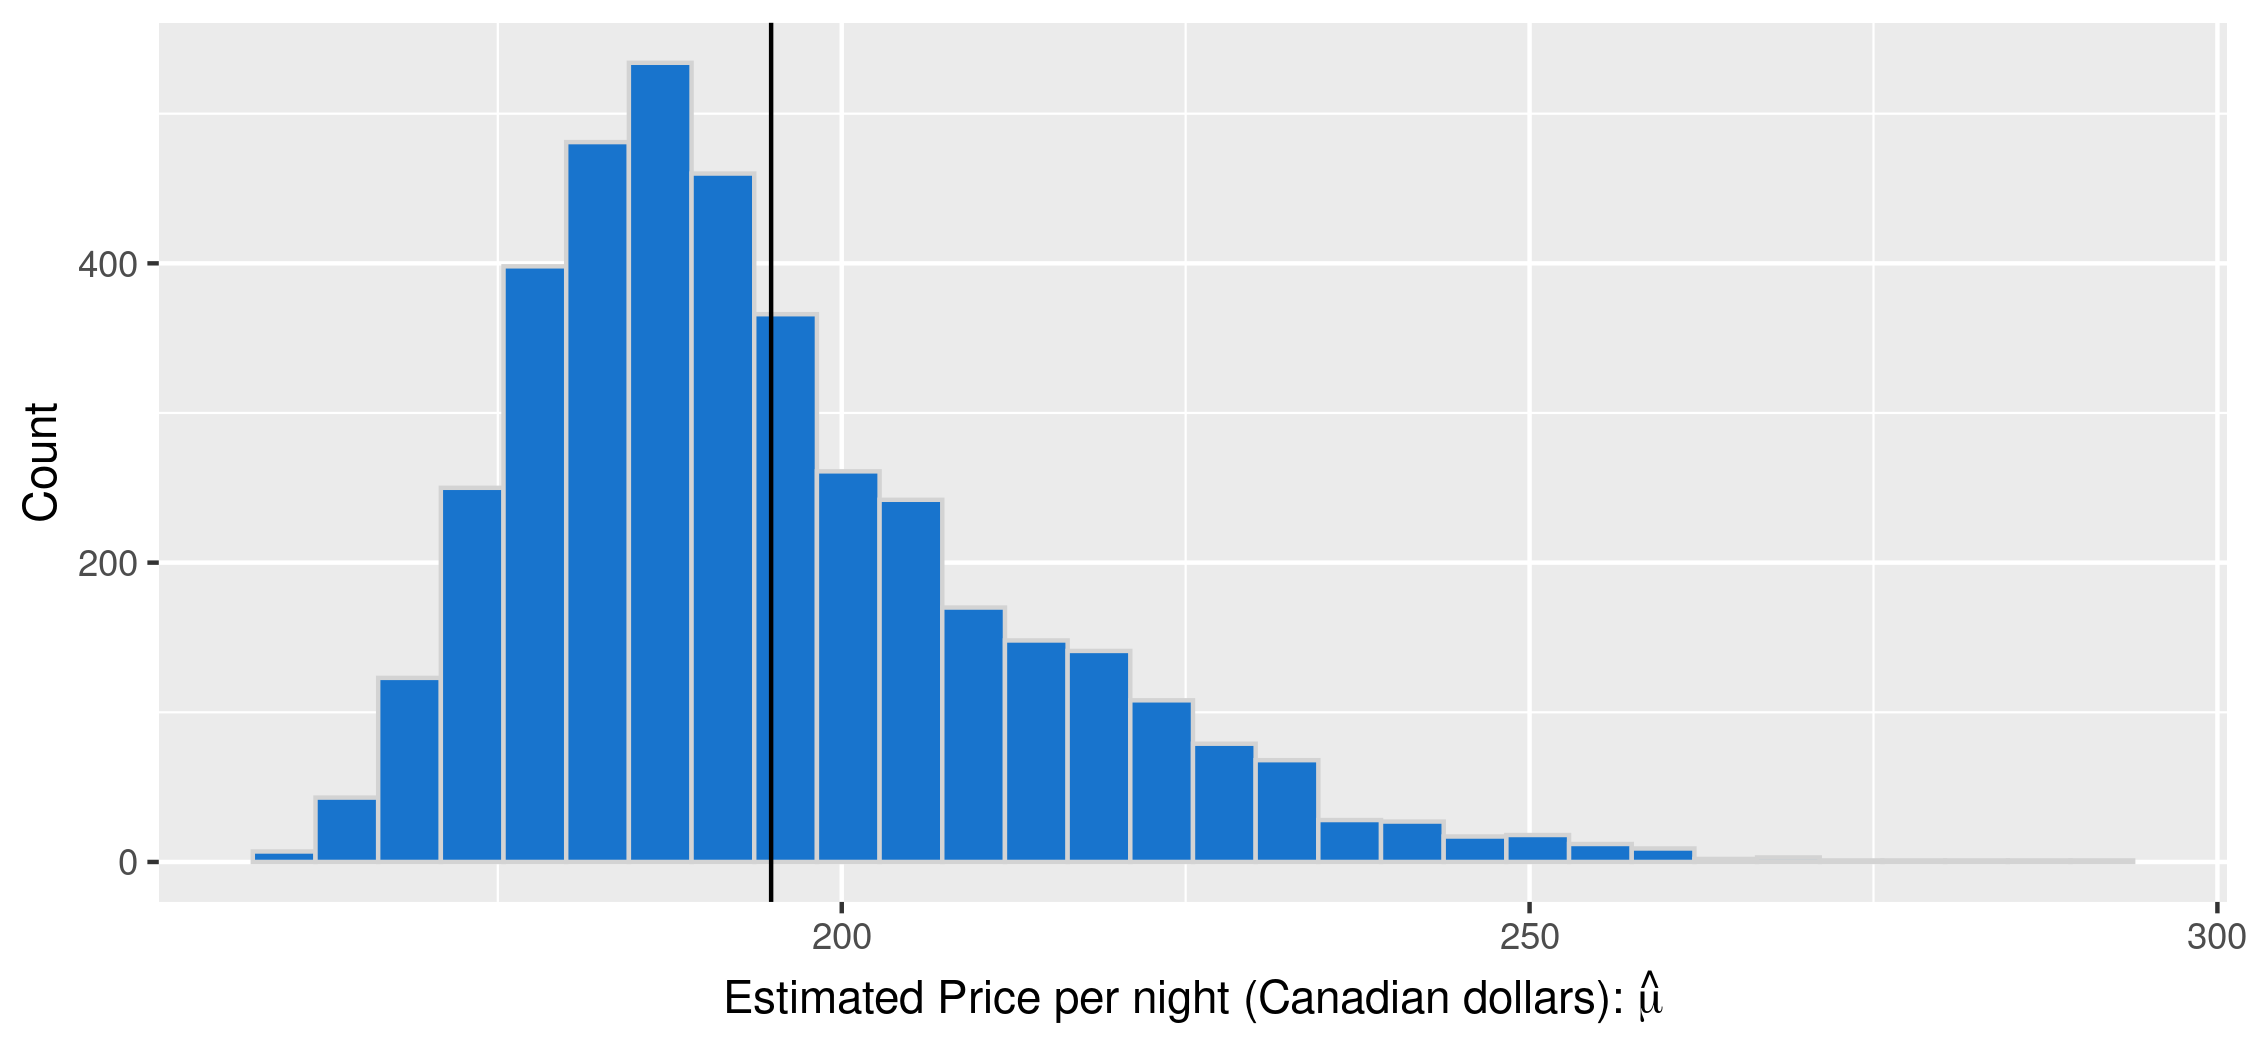
\includegraphics[width=0.98\linewidth,height=0.461\linewidth]{figure/base-hist-1} 

}



\end{knitrout}
}


\newcommand{\BaseHistogramWithArrow}{
\begin{knitrout}
\definecolor{shadecolor}{rgb}{0.969, 0.969, 0.969}\color{fgcolor}

{\centering 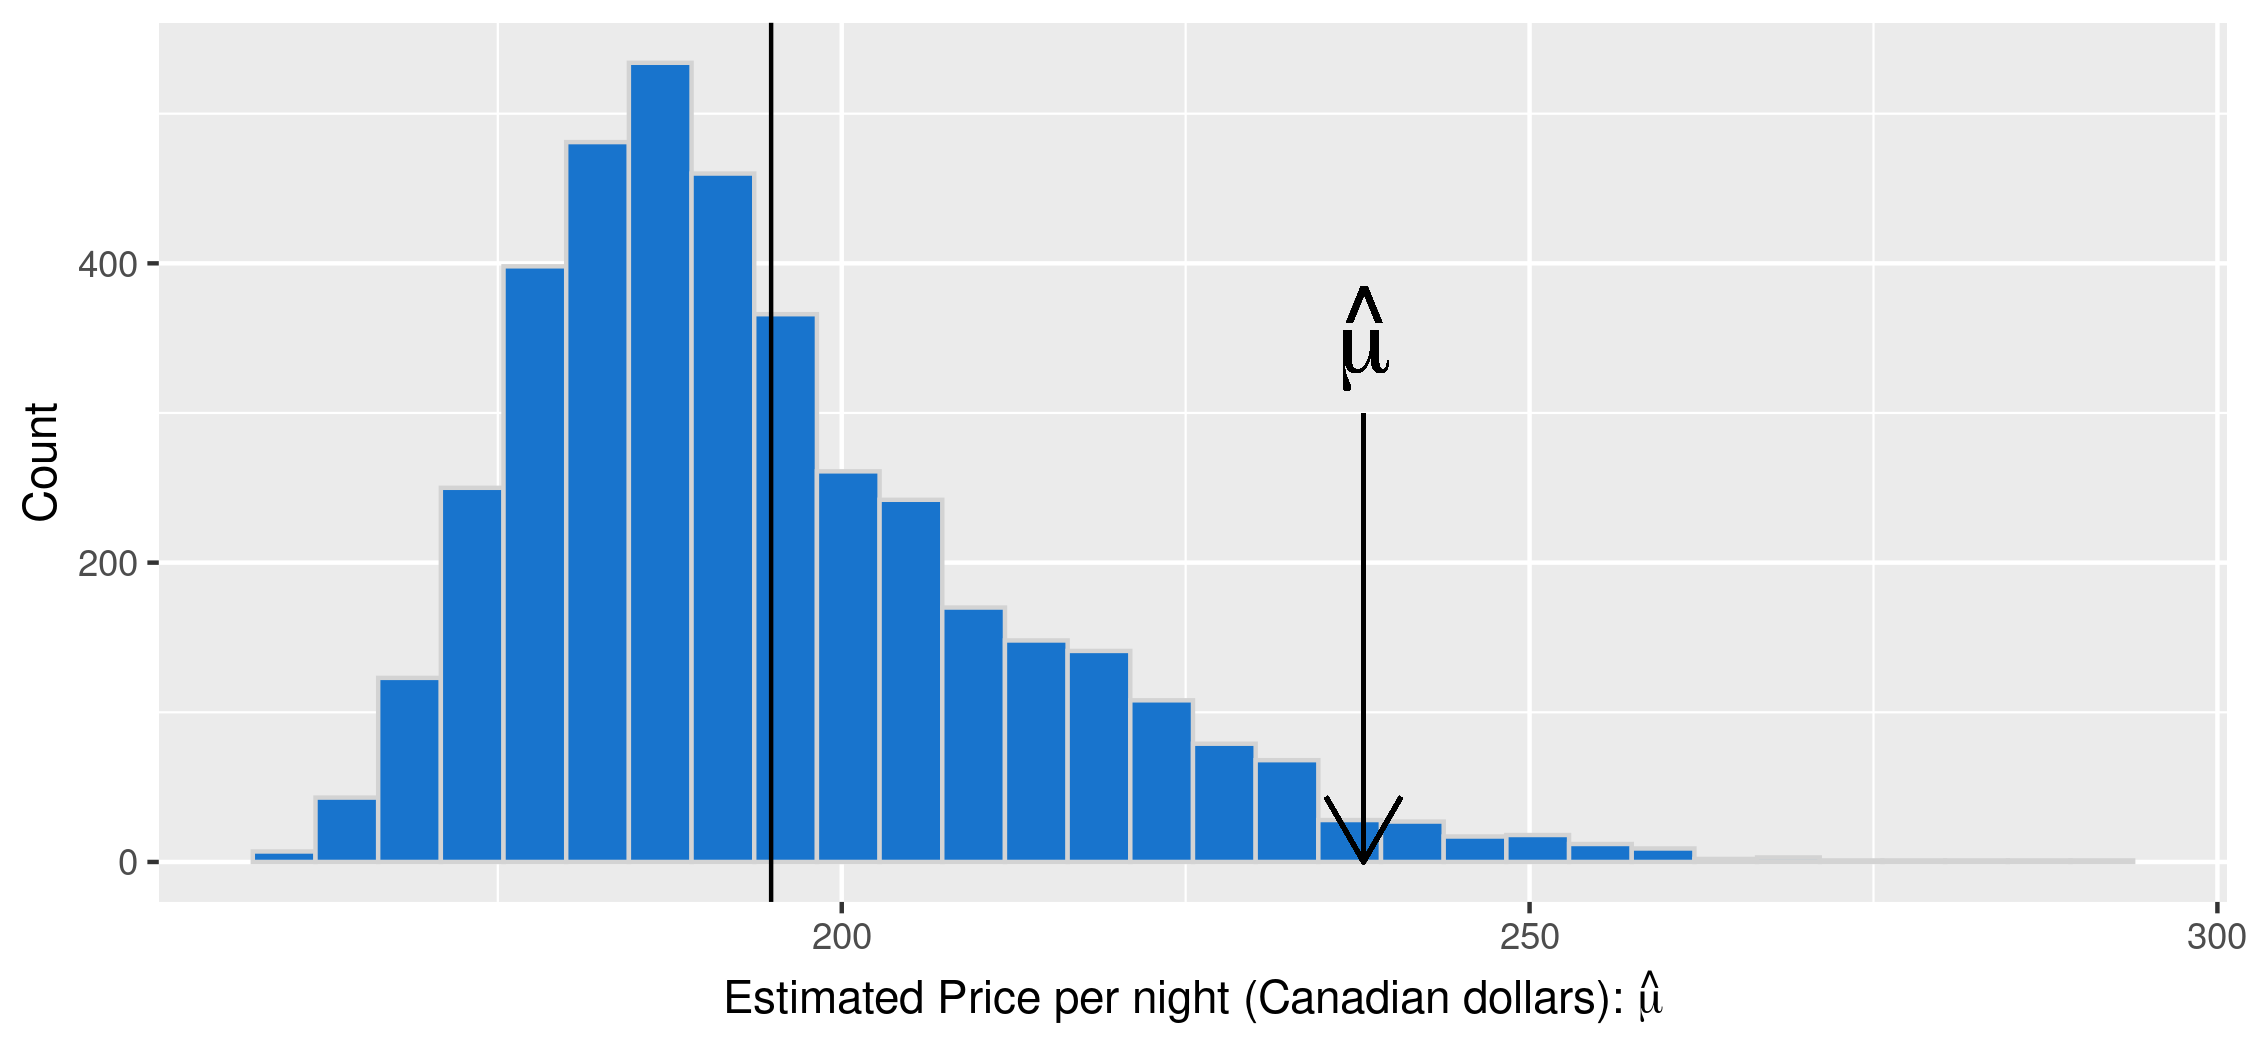
\includegraphics[width=0.98\linewidth,height=0.461\linewidth]{figure/base-hist-arrow-1} 

}



\end{knitrout}
}



\newcommand{\BaseHistogramFaded}{
\begin{knitrout}
\definecolor{shadecolor}{rgb}{0.969, 0.969, 0.969}\color{fgcolor}

{\centering 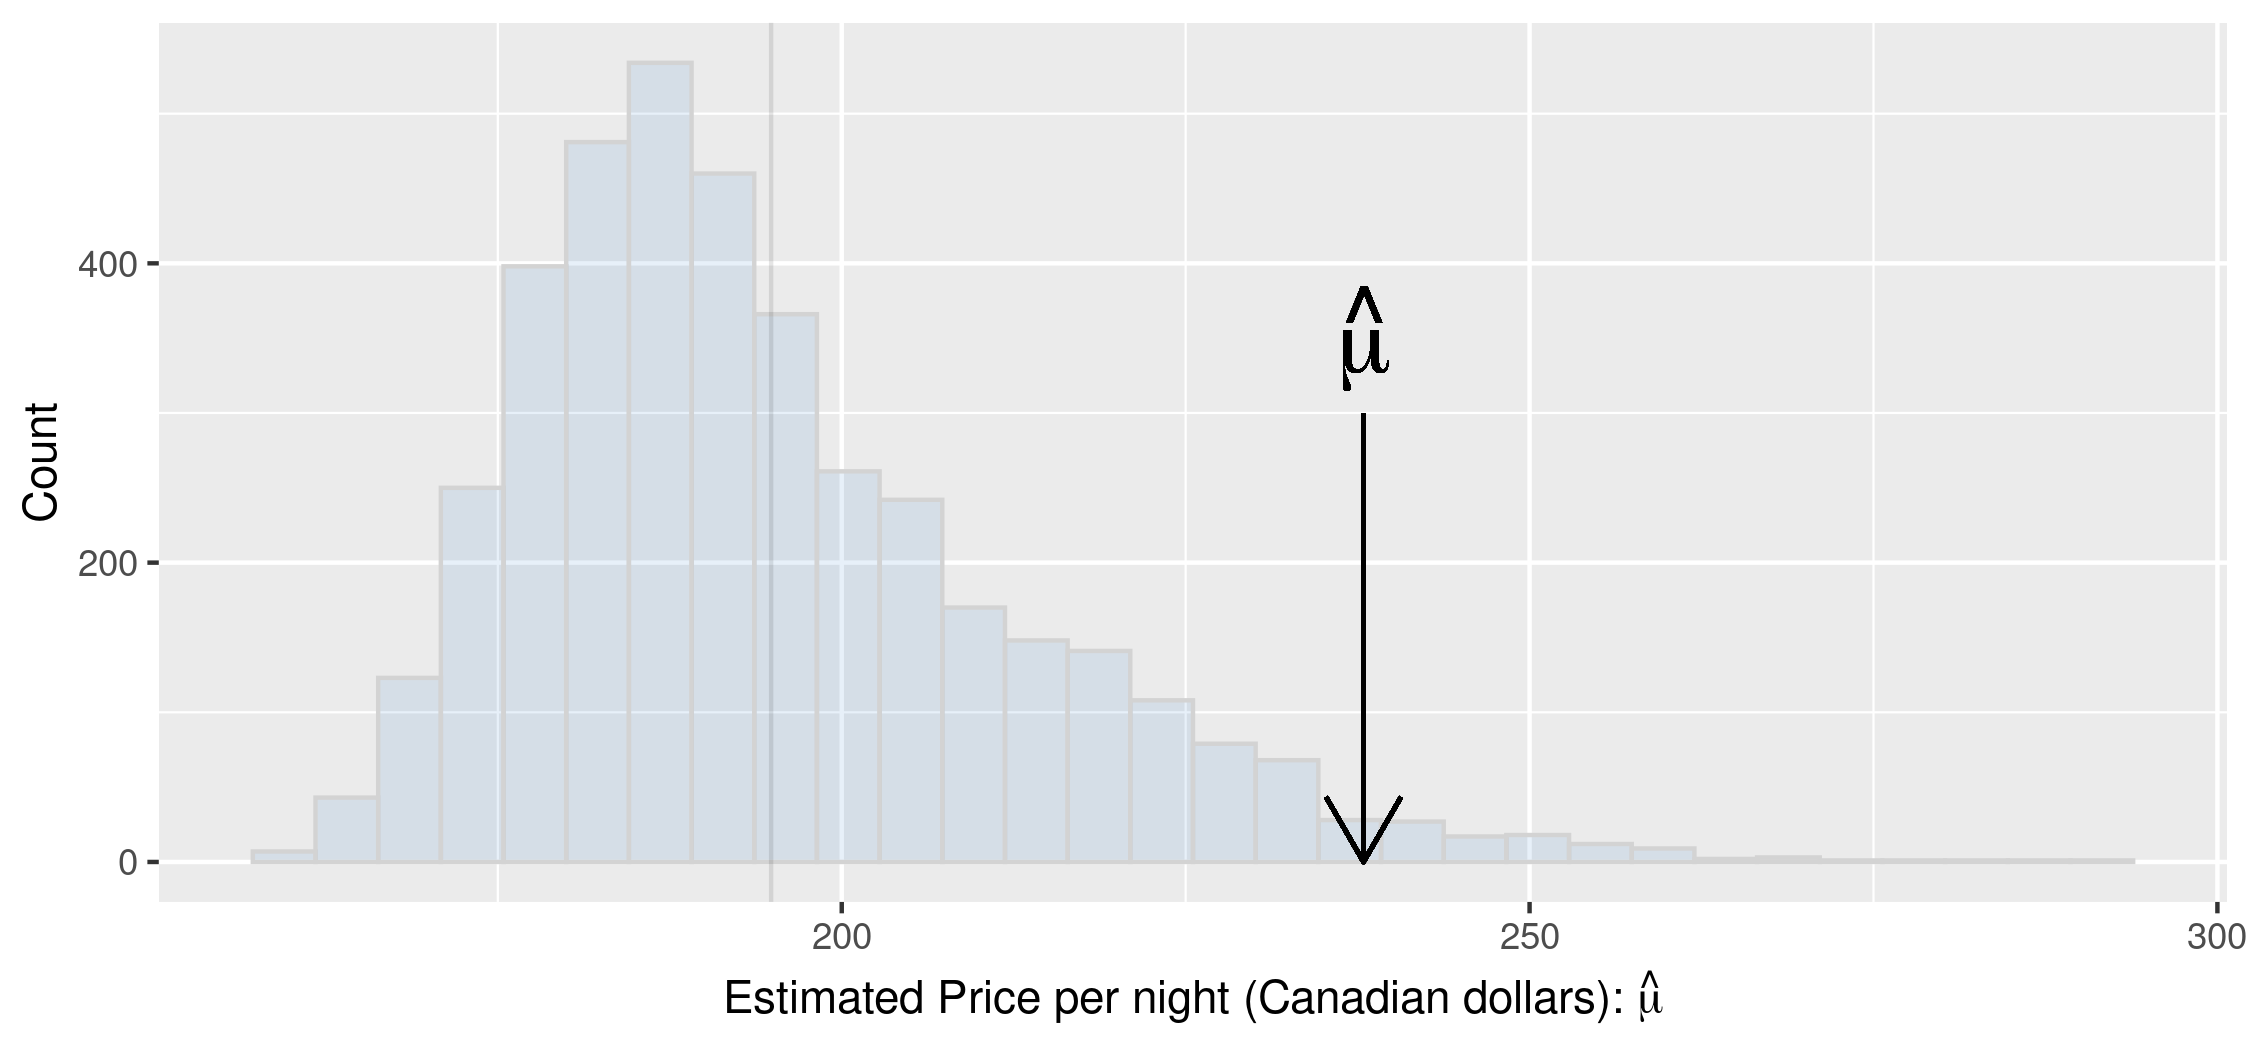
\includegraphics[width=0.98\linewidth,height=0.461\linewidth]{figure/base-hist-faded-1} 

}



\end{knitrout}
}


\newcommand{\SingleCI}{
\begin{knitrout}
\definecolor{shadecolor}{rgb}{0.969, 0.969, 0.969}\color{fgcolor}

{\centering 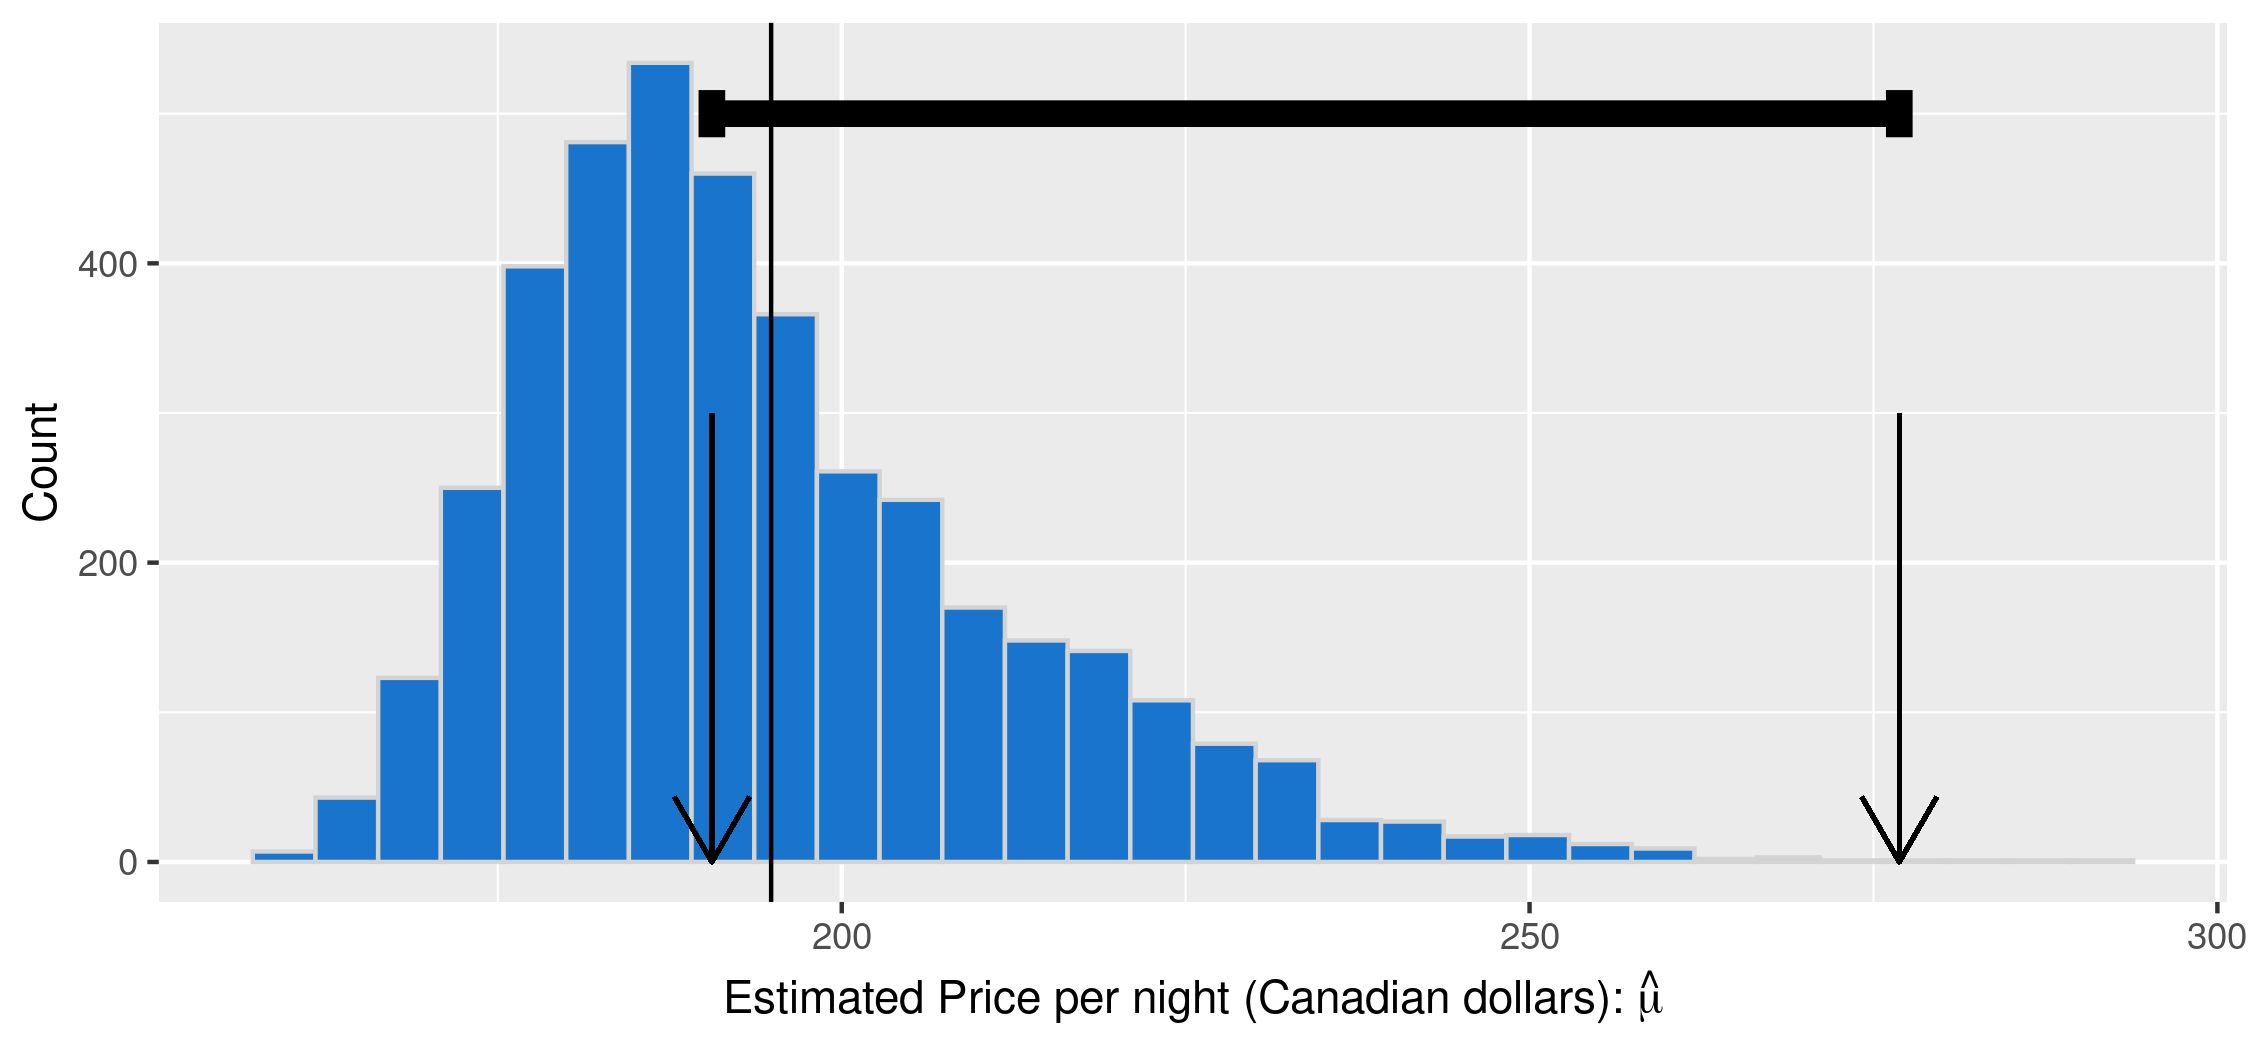
\includegraphics[width=0.98\linewidth,height=0.461\linewidth]{figure/base-hist-ci-1} 

}



\end{knitrout}
}




\newcommand{\SingleCIB}{
\begin{knitrout}
\definecolor{shadecolor}{rgb}{0.969, 0.969, 0.969}\color{fgcolor}

{\centering 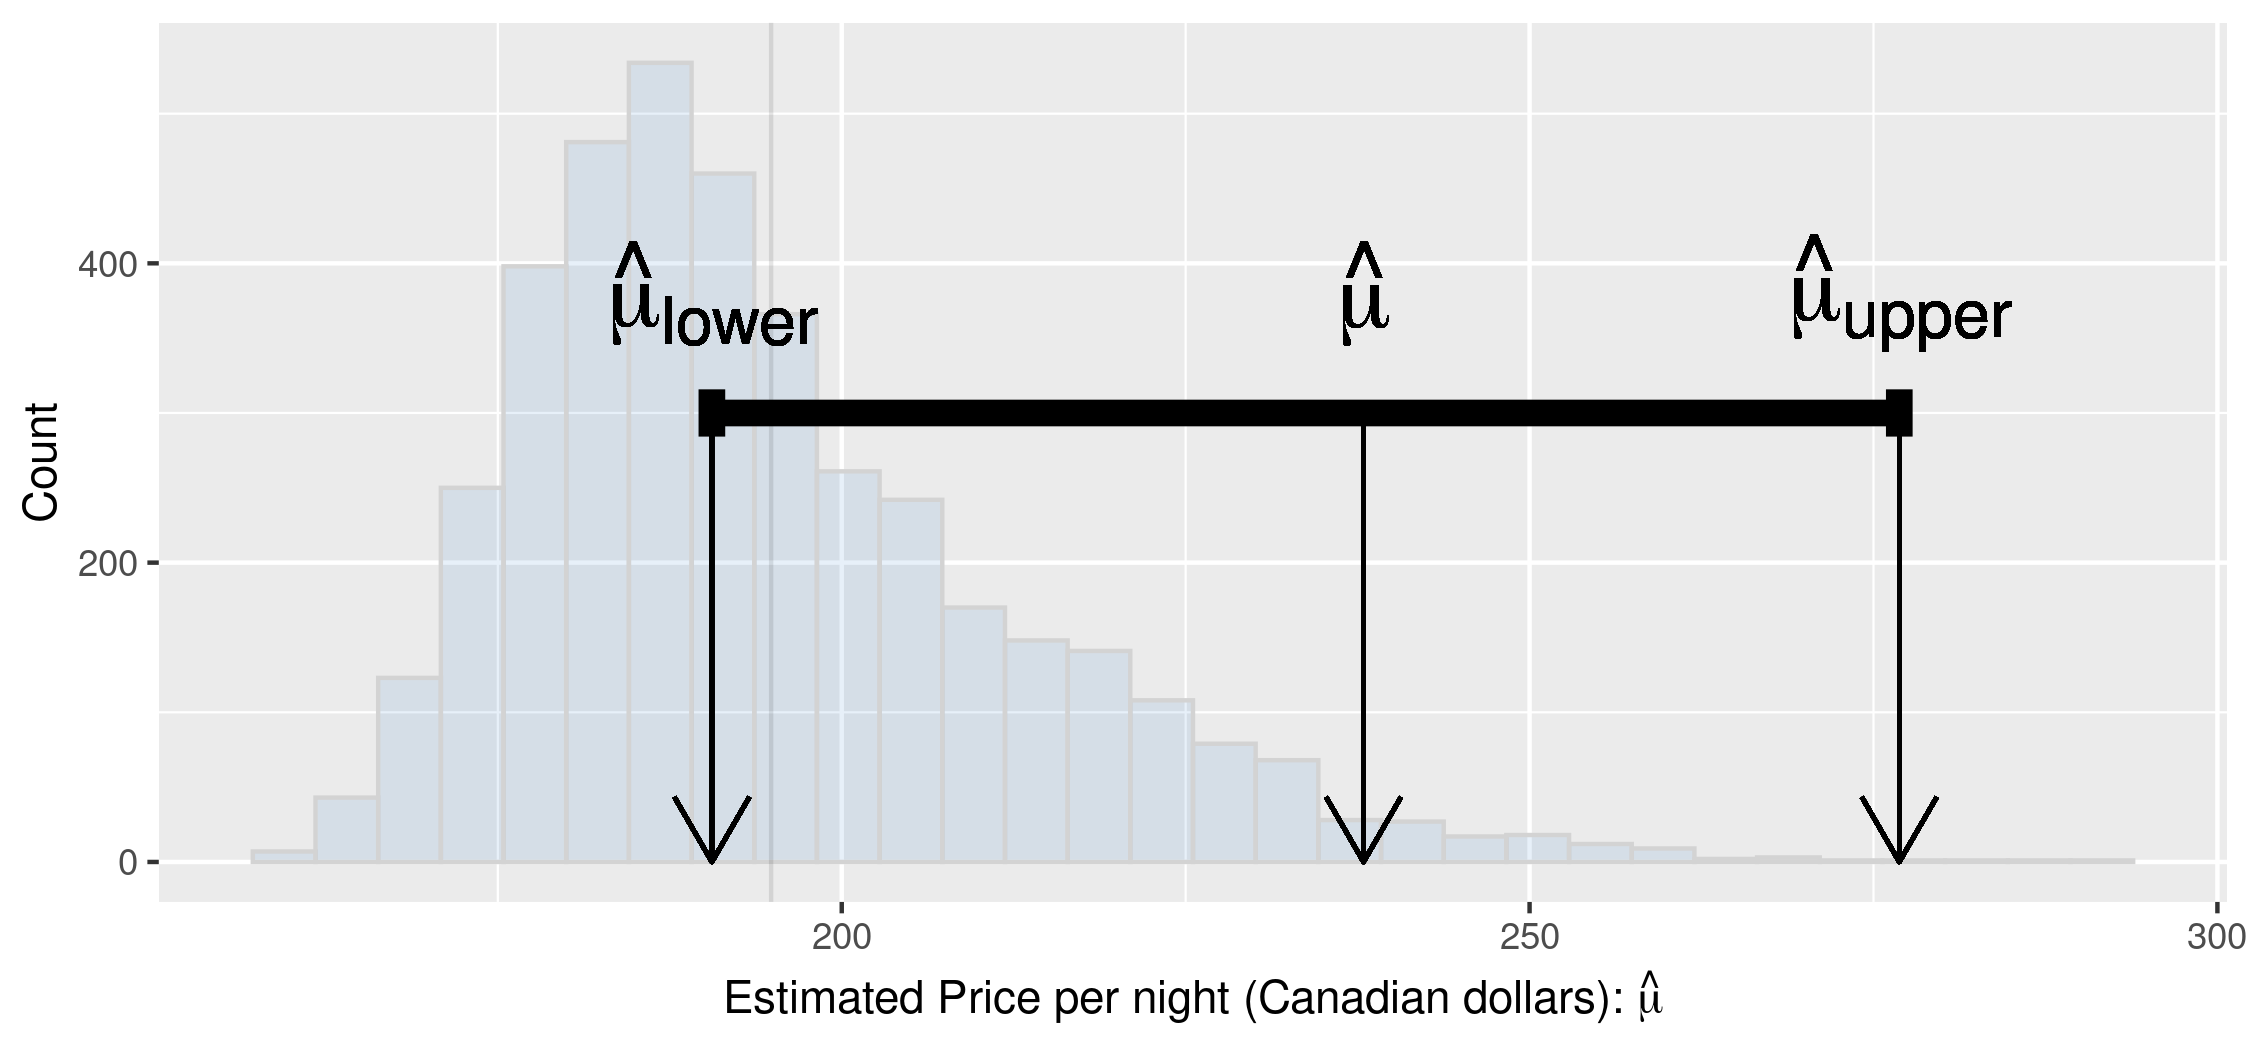
\includegraphics[width=0.98\linewidth,height=0.461\linewidth]{figure/base-hist-cib-1} 

}



\end{knitrout}
}



\newcommand{\MultipleCIs}{



\begin{knitrout}
\definecolor{shadecolor}{rgb}{0.969, 0.969, 0.969}\color{fgcolor}

{\centering 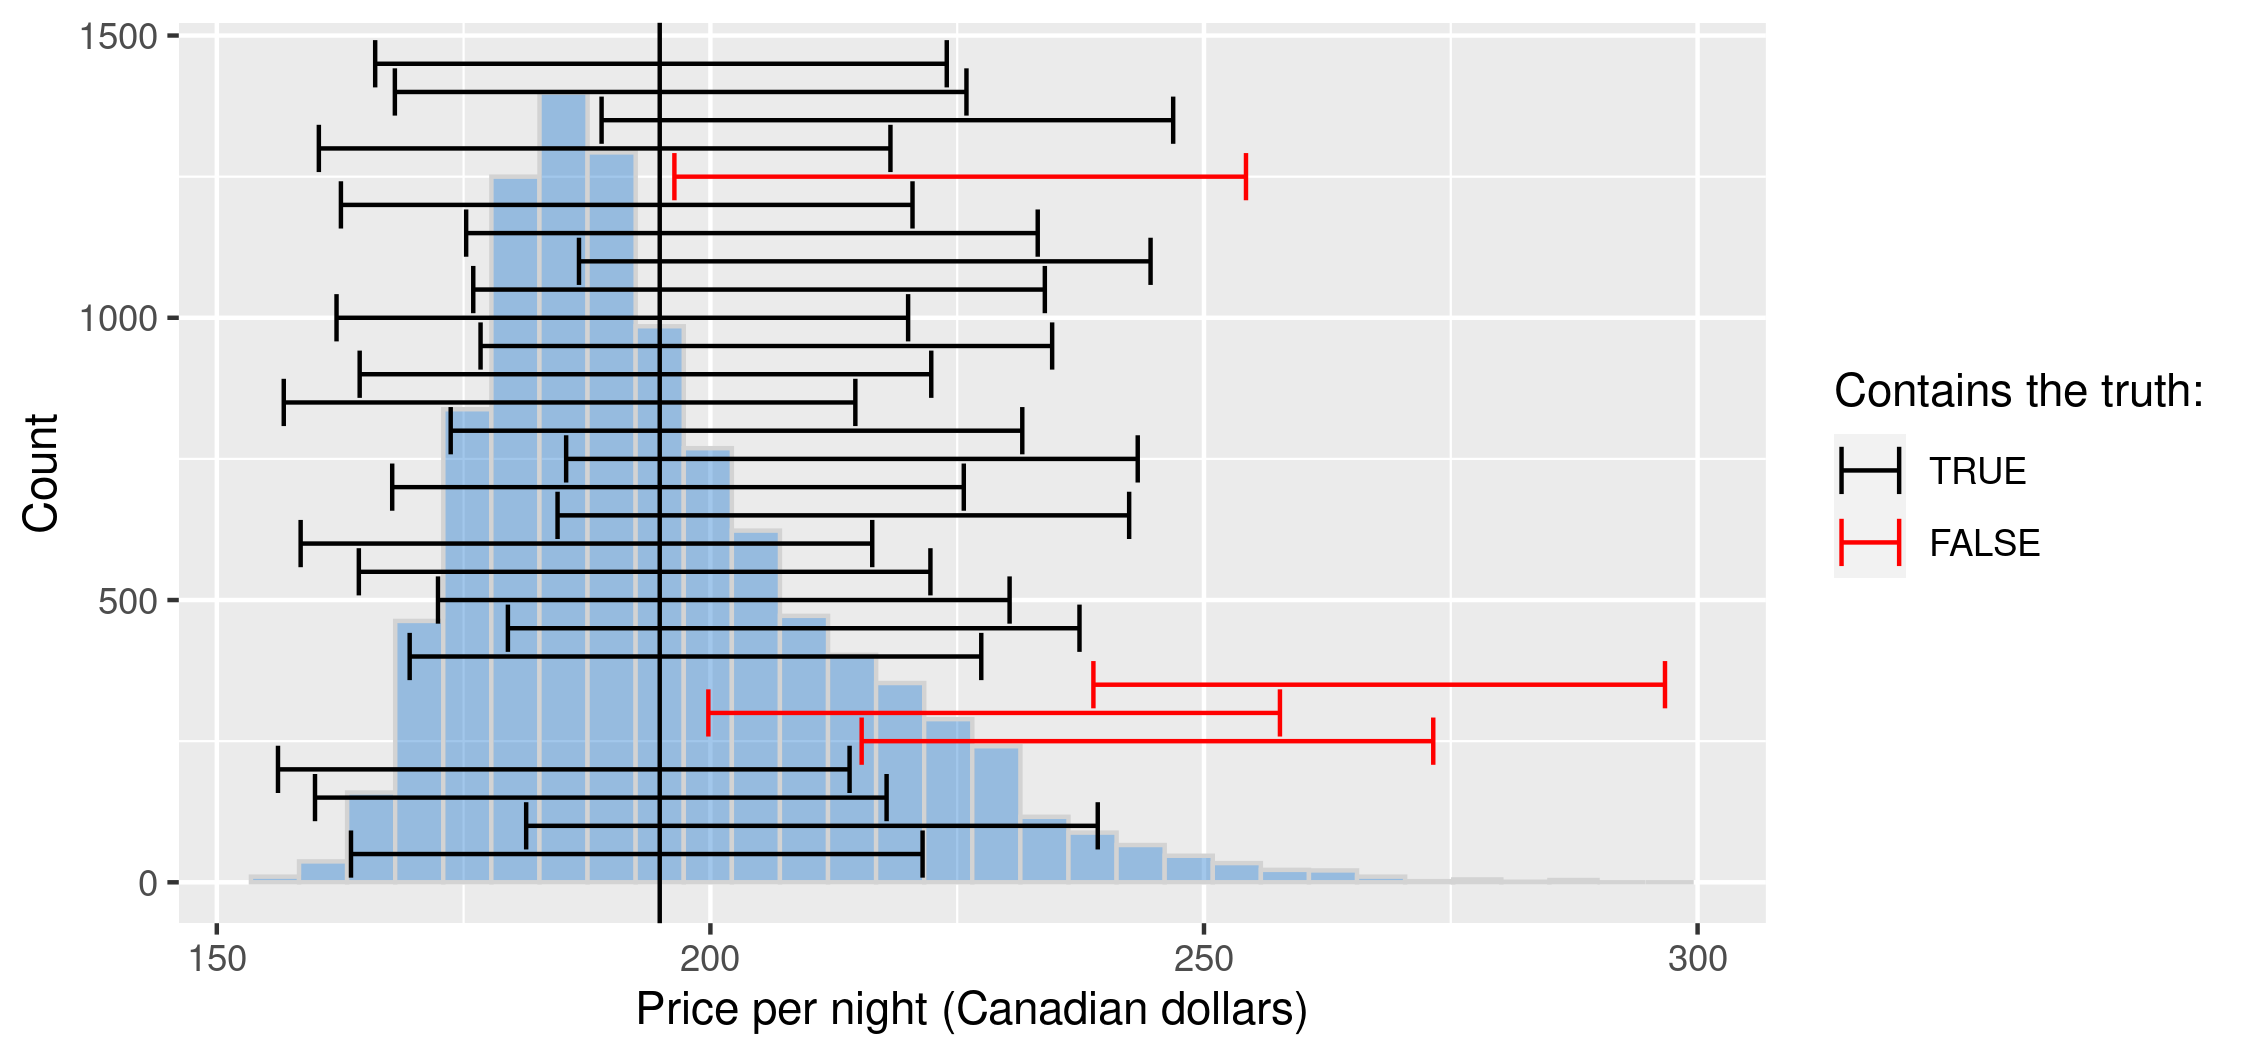
\includegraphics[width=0.98\linewidth,height=0.461\linewidth]{figure/base-hist-cis-1} 

}



\end{knitrout}
}



\title{Local Weighting--Based Diagnostics for Bayesian Poststratification}
\author{Ryan Giordano, Alice Cima, Erin Hartman, Jared Murray, Avi Feller}

\date{\textbf{Berkeley BSTARS September 2025}}

\setbeamertemplate{Collaborators}[none]
\IfFileExists{upquote.sty}{\usepackage{upquote}}{}

\begin{document}

\maketitle


\begin{frame}{Mister freakin P}


\end{frame}






\begin{frame}{The basic problem}

%\adjincludegraphics[width=0.9\textwidth,trim={0 {.5\height} 0 0 }, clip]{static_figures/survey_and_voting.jpg}

We have a survey population, for whom we observe:
%
\begin{itemize}
 \item Covariates $\x$ (e.g.~race, gender, zip code, age, education level)
 \item Responses $\y$ (e.g.~A binary response to ``do you support policy such--and--such'')
\end{itemize}
%

We want the average response in a target population,
in which we observe only covariates.



\splitpage{
    \centering
    \only<1>{
    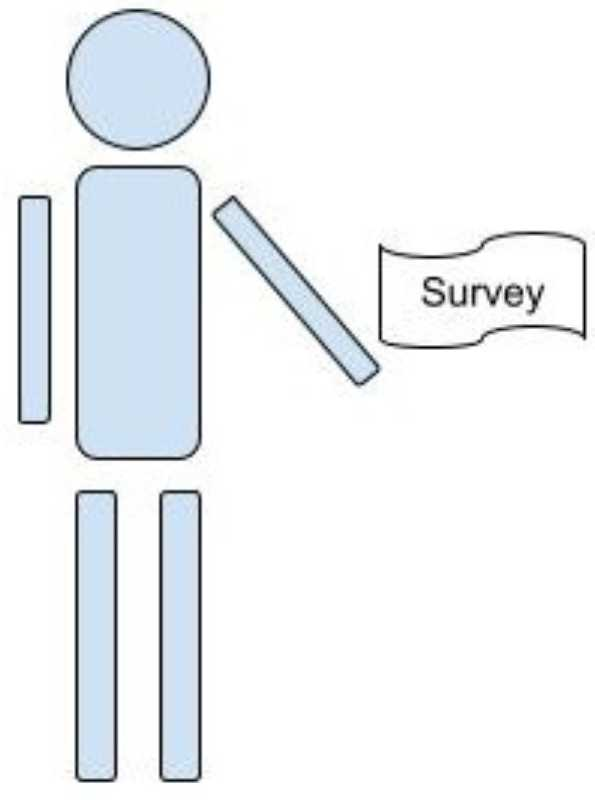
\includegraphics[width=0.5\textwidth]{static_figures/survey_man.jpg}
    }
    \only<2->{
    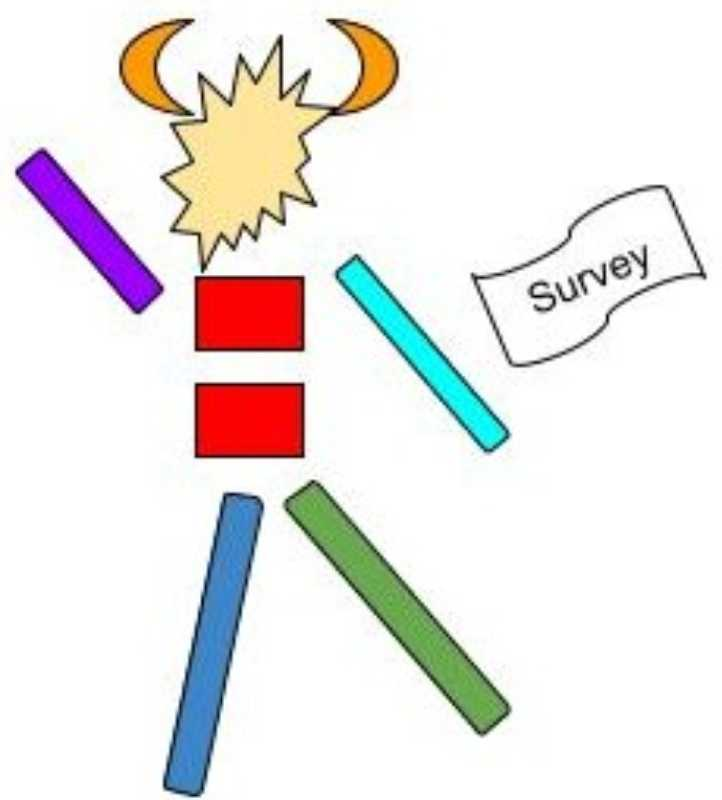
\includegraphics[width=0.5\textwidth]{static_figures/survey_crazy_man.jpg}
    }
}{
    \centering
    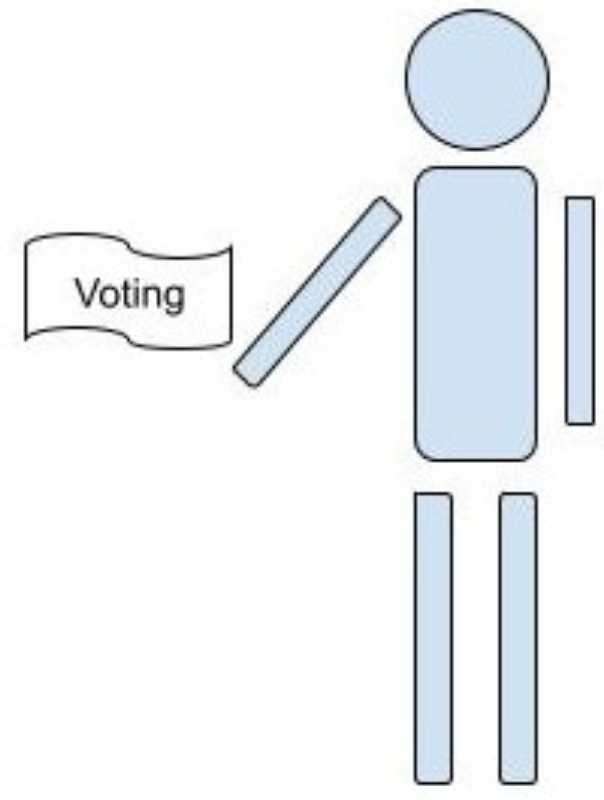
\includegraphics[width=0.5\textwidth]{static_figures/voting_man.jpg}
}

\splitpage{
    \centering
    Observe $(\x_s, y_s)$ for $s = 1, \ldots, \nsur$\\
}{
    \centering
    Observe $\x_p$ for $p = 1, \ldots, \ntar$\\
}

\onslide<2->{
\textbf{The problem is that the populations are very different.}
}

\onslide<3->{
    Our survey results may be biased.

    How can we use the covariates
    to say something about the target responses?
}
%
\end{frame}

%%%%%%%%%%%%%%%%%%%%%%%%%%%%%%%%%%%%%%%%%%%%%%%%%%%%%%%
%%%%%%%%%%%%%%%%%%%%%%%%%%%%%%%%%%%%%%%%%%%%%%%%%%%%%%%
%%%%%%%%%%%%%%%%%%%%%%%%%%%%%%%%%%%%%%%%%%%%%%%%%%%%%%%

\begin{frame}[t]{Two approaches}

We want $\mu := \meantar \y_p$, but don't observe $\y_p$ in the target population.

\begin{itemize}
    \item Assume $p(y | x)$ is the same in both populations,
    \item But the distribution of $x$ may be different in the survey and target.
\end{itemize}
%

\splitpage{
    \centering
    \textbf{Calibration weighting}
}{
    \centering
    \textbf{Bayesian hierarchical modeling (MrP)}
}

\splitpage{
    \centering
    Choose ``calibration weights'' $w_s$\\
    (e.g.~raking weights)
}{
    \centering
    Choose a model $\p(\y | x, \theta)$ and prior $\p(\theta)$\\
    (e.g.~Hierarchical logitstic regression)
}

\splitpage{
    \centering
    $\muhat_{\cal} = \meansur w_s y_s$
}{
    \centering
    Take $\yhat_p = \expect{\p(\theta \vert \textrm{Survey data})}{\y | \x_p}$ and\\
    $\muhat_{\mrp} = \meantar \yhat_p$
}

\splitpage{
    \centering
    Dependence on $\y_s$ is obvious\\
    ($\w_s$ typically chosen using only $\x$)
}{
    \centering
    Dependence on $\y_s$ very complicated\\
    (Typically via MCMC draws from $\p(\theta \vert \textrm{Survey data})$)
}

\splitpage{
    \centering
    Weights give interpretable diagnostics:
    %
    \begin{itemize}
        \item Frequentist variability
        \item Partial pooling
        \item Regressor balance
    \end{itemize}
    %
}{
    \centering
    \textbf{Black box}
}

We open the MrP black box, and provide versions of all these diagnostics,
for nonlinear hierarchical models fit with MCMC.

\end{frame}



%%%%%%%%%%%%%%%%%%%%%%%%%%%%%%%%%%%%%%%%%%%%%%%%%%%%%%%
%%%%%%%%%%%%%%%%%%%%%%%%%%%%%%%%%%%%%%%%%%%%%%%%%%%%%%%
%%%%%%%%%%%%%%%%%%%%%%%%%%%%%%%%%%%%%%%%%%%%%%%%%%%%%%%

\begin{frame}[t]{Covariate balance}

What do we want out of calibration weights?

$$
\textrm{Target average} =
\meantar \y_p \approx \meansur \w_s \y_s
= \textrm{Weighted survey average}
$$

We can't check this, because we don't observe $\y_p$.  But we can check
whether

$$
% \textrm{Target average regeressor} =
    \meantar \x_p = \meansur \w_s \x_s
% =    \textrm{Weighted survey average regressor}
$$

Such weights satisfy ``covariate balance'' for $\x$.

You can check covariate balance for any calibration weighting estimator.

Even more, covariate balance is the criterion for a popular class of calibration
weight estimators:

\begin{block}{Raking calibration weights}
% Select calibration weights to satisfy
$$
\begin{aligned}
    \textrm{ Take }
    \w_1, \ldots, \w_{\Nsur} :={}& \argmin \sumsur (\w_s - \w_s^{\mathrm{ref}})^2 \\
    \textrm{Subject to }
    \meantar f(\x_p) ={}& \meansur \w_s f(\x_s)
    \textrm{ for some function }f(\cdot).
\end{aligned}
$$
\end{block}



\end{frame}




%%%%%%%%%%%%%%%%%%%%%%%%%%%%%%%%%%%%%%%%%%%%%%%%%%%%%%%
%%%%%%%%%%%%%%%%%%%%%%%%%%%%%%%%%%%%%%%%%%%%%%%%%%%%%%%
%%%%%%%%%%%%%%%%%%%%%%%%%%%%%%%%%%%%%%%%%%%%%%%%%%%%%%%

\begin{frame}[t]{Covariate balance}

Why would you want covariate balance?  Some commonly stated reasons:

%
\begin{itemize}
\item To reduce the variance of inverse propensity weights (IPW)
\item To check the accuracy of IPW
\item To exactly balance ``important regressors''
\end{itemize}
%
Common to these motivations is the following concen:

% \begin{block}{Why covariate balance?}
    We want to balance $f(\x)$ because we think
    $\expect{}{\y \vert \x}$ might plausibly vary $\propto f(\x)$.
    % \\[1em]

    Covariate balance ensures that such variation is captured
    by our calibration estimator.
% \end{block}


\begin{block}{General covariate balance check}
    Pick a small $\delta$, and define a \emph{new response variable} $\ytil$ such that
    $$
    \expect{}{\ytil \vert \x} = \expect{}{\y \vert \x} + \delta f(\x).
    $$
    We know the change this perturbation produces in the target distribution:
    $$
    \mu(\ytil) - \mu(\y) = \delta \meantar f(\x_p)
    $$
    Covariate balance for an estimator $\muhat$ checks whether
    $\muhat(\ytil) - \muhat(\y) = \mu(\ytil) - \mu(\y)$.
\end{block}


\end{frame}



%%%%%%%%%%%%%%%%%%%%%%%%%%%%%%%%%%%%%%%%%%%%%%%%%%%%%%%
%%%%%%%%%%%%%%%%%%%%%%%%%%%%%%%%%%%%%%%%%%%%%%%%%%%%%%%
%%%%%%%%%%%%%%%%%%%%%%%%%%%%%%%%%%%%%%%%%%%%%%%%%%%%%%%

\begin{frame}[t]{MrPaw}

How to form a notion of covariate balance for estimators that are not weighted averages?

\splitpage{
    \centering
    \textbf{Calibration weights}\\
    $\muhat_{\cal} = \meansur w_s y_s$
}{
    \centering
    \textbf{MrP}\\
    Take $\yhat_p = \expect{\p(\theta \vert \textrm{Survey data})}{\y | \x_p}$ and\\
    $\muhat_{\mrp} = \meantar \yhat_p$
}


\vspace{1em}
\hrulefill\\
\textbf{Step one: Define weights.}

Noting that $w_s = \frac{d}{d \y_s} \muhat_{\cal}$, we can define

$$
\wmrp_s := \frac{d}{d\y_s} \muhat_{\mrp}. %= \meantar \frac{d}{d\y_s} \yhat_p.
$$

It happens that the needed derivatives are given
by simple a posterior covariances involving only the inverse
link function $m(\x; \theta)$ and
log likelihood \citep{giordano:2018:covariances}:

$$
\frac{d \yhat_p}{d\y_s}  =
    \cov{\p(\theta \vert \textrm{Survey data})}{
        m(\x_p; \theta),
        \frac{\partial}{\partial \y} \log p(\y \vert \theta, \x_s)}
$$

These can be computed using standard MCMC software \citep{brms}.

No other weight definition will do --- in some cases,
MrP is exactly a calibration estimator (e.g. linear regression with flat priors),
and we want the definitions to coincide in that case.

\end{frame}



%%%%%%%%%%%%%%%%%%%%%%%%%%%%%%%%%%%%%%%%%%%%%%%%%%%%%%%
%%%%%%%%%%%%%%%%%%%%%%%%%%%%%%%%%%%%%%%%%%%%%%%%%%%%%%%
%%%%%%%%%%%%%%%%%%%%%%%%%%%%%%%%%%%%%%%%%%%%%%%%%%%%%%%

\begin{frame}[t]{Covariate balance}


How to form a notion of covariate balance for estimators that are not weighted averages?

\splitpage{
    \centering
    \textbf{Calibration weights}\\
    $\muhat_{\cal} = \meansur w_s y_s$
}{
    \centering
    \textbf{MrP}\\
    Take $\yhat_p = \expect{\p(\theta \vert \textrm{Survey data})}{\y | \x_p}$ and\\
    $\muhat_{\mrp} = \meantar \yhat_p$
}

\vspace{1em}
\hrulefill\\
\textbf{Step two: Specify a Taylor series.}

\def\new{\mathrm{new}}
Suppose we wanted to re--compute MrP with new
survey responses $\y_s^{\new}$.

$$
\muhat_{\mrp}(\y_1^\new, \ldots, \y_{\nsur}^\new) =
\sumsur \w_s^\mrp (\y_s^\new  - \y_s) + \mathrm{Residual}
$$

In general, MrP is truly nonlinear. The residual is only small when $\y_s^\new \approx \y_s$!


\end{frame}


%%%%%%%%%%%%%%%%%%%%%%%%%%%%%%%%%%%%%%%%%%%%%%%%%%%%%%%
%%%%%%%%%%%%%%%%%%%%%%%%%%%%%%%%%%%%%%%%%%%%%%%%%%%%%%%
%%%%%%%%%%%%%%%%%%%%%%%%%%%%%%%%%%%%%%%%%%%%%%%%%%%%%%%

\begin{frame}[t]{Covariate balance}


How to form a notion of covariate balance for estimators that are not weighted averages?

\splitpage{
    \centering
    \textbf{Calibration weights}\\
    $\muhat_{\cal} = \meansur w_s y_s$
}{
    \centering
    \textbf{MrP}\\
    Take $\yhat_p = \expect{\p(\theta \vert \textrm{Survey data})}{\y | \x_p}$ and\\
    $\muhat_{\mrp} = \meantar \yhat_p$
}

\vspace{1em}
\hrulefill\\
\textbf{Step three: Define a data perturbation that captures regression balance.}



\end{frame}






%%%%%%%%%%%%%%%%%%%%%%%%%%%%%%%%%%%%%%%%%%%%%%%%%%%%%%%
%%%%%%%%%%%%%%%%%%%%%%%%%%%%%%%%%%%%%%%%%%%%%%%%%%%%%%%
%%%%%%%%%%%%%%%%%%%%%%%%%%%%%%%%%%%%%%%%%%%%%%%%%%%%%%%

\begin{frame}[t]{Generalized covariate balance for MrP}

\textbf{Step one:} Construct
$\ytil$ such that $\expect{}{\ytil \vert \x} = \expect{}{\y \vert \x} + \delta f(\x)$.
\pause

\textbf{Problem:} Our $\y$ is binary!  (We're motivated by hierarchical linear regression.)

\pause
Two possibilities:
%
\begin{itemize}
    \item Allow $\ytil$ to take values other than $\{0,1\}$ and set
        $\ytil = \y + \delta \f(\x)$, or
    \item Use an estimate of $\expect{}{\y \vert \x}$ to draw new binary $\ytil$.
\end{itemize}
%
Our approach:
%
\begin{itemize}
    \item Use $\ytil = \y + \delta \f(\x)$ to identify problematic ``imbalanced'' $\f(\x)$
    \item Sanity check by generating binary $\ytil$ using $\f(\x)$ (which is fast and easy)
\end{itemize}


\end{frame}



%%%%%%%%%%%%%%%%%%%%%%%%%%%%%%%%%%%%%%%%%%%%%%%%%%%%%%%
%%%%%%%%%%%%%%%%%%%%%%%%%%%%%%%%%%%%%%%%%%%%%%%%%%%%%%%
%%%%%%%%%%%%%%%%%%%%%%%%%%%%%%%%%%%%%%%%%%%%%%%%%%%%%%%

\begin{frame}[t]{Generalized covariate balance for MrP}

\textbf{Step one:} Construct
$\ytil$ such that $\expect{}{\ytil \vert \x} = \expect{}{\y \vert \x} + \delta f(\x)$.\\
\pause
\textbf{Step two:} Evaluate \surcol{$\muhat_\mrp(\ytil) - \muhat(\y)$}.
\pause

\textbf{Problem:} \surcol{$\muhat_\mrp(\cdot)$} is computed with MCMC.
%
\begin{itemize}
\item Each MCMC run typically takes hours, and
\item Output is noisy, and \surcol{$\muhat_\mrp(\ytil) - \muhat(\y)$} may be small.
\end{itemize}
%

\pause
\begin{block}{MrP Local Equivalent Weights (MrPlew)}
Form the approximation
\surcol{
$$
\muhat_{\mrp}(\ytil) =
    \sumsur \w_i^\mrp (\ytil_i  - \y_i) + \mathrm{Residual}
\quad\textrm{where}\quad
    \wmrp_i := \frac{d}{d\y_i} \muhat_{\mrp}(\y). %= \meantar \frac{d}{d\y_s} \yhat_p.
$$
}
\end{block}

\only<5>{
    \textbf{Computation: }
The weights are given by weighted averages of posterior covariances  \footcite{giordano:2018:covariances}.
\\[1em]
They can be easily computed with standard software\footnote{We use \texttt{brms} \parencite{brms}.}
\textbf{without re--running MCMC}.\\
}


\only<6>{
    %
    \textbf{Theory: }
We state conditions under which, as $\delta \rightarrow 0$, and $N \rightarrow \infty$,
\begin{itemize}
\item The residual is of lower order than the MrPlew term,
\item \textit{Uniformly} over a very wide class of $\f(\cdot)$.
\end{itemize}
%
\textbf{Uniformity} is the hard part, but this justifies
using MrPlew to \textit{identify} problematic $\f(\cdot)$.

Builds on earlier work on uniform error bounds
for Bernstein--von Mises theorem(--ish) results
\footcite{giordano:2024:bayesij,kasprzak:2025:laplace}.
}


\only<7>{
If MrP were linear (e.g.~if you use OLS instead of hierarchical
logistic regression), then
%
\begin{itemize}
\item The residual is zero,
\item $\muhat_{\mrp}(\y) = \sumsur \w_i^\mrp \y_i$, and so
\item $\muhat_{\mrp}(\ytil)$ is a calibration weighting
estimator, and $\wmrp_i$ are its weights.  (Cite Gelman)
\end{itemize}
%
In general, MrP is truly nonlinear. The residual is only small when $\ytil \approx \y$
(i.e., when $\delta \ll 1$).
}




\end{frame}





\begin{frame}{Experiment}

Show using the Alexander experiment that
%
\begin{itemize}
    \item The MrPaw approximation is accurate, even up to a standard deviation away
    \item Differential imbalance actually exists between raking and MrP and we can detect it
    \item We can make binary datasets for the changes, and there's variability in how to do that
\end{itemize}
%
Remind that we can do frequentist variance and partial pooling too.

\end{frame}

\begin{frame}{Experiment}
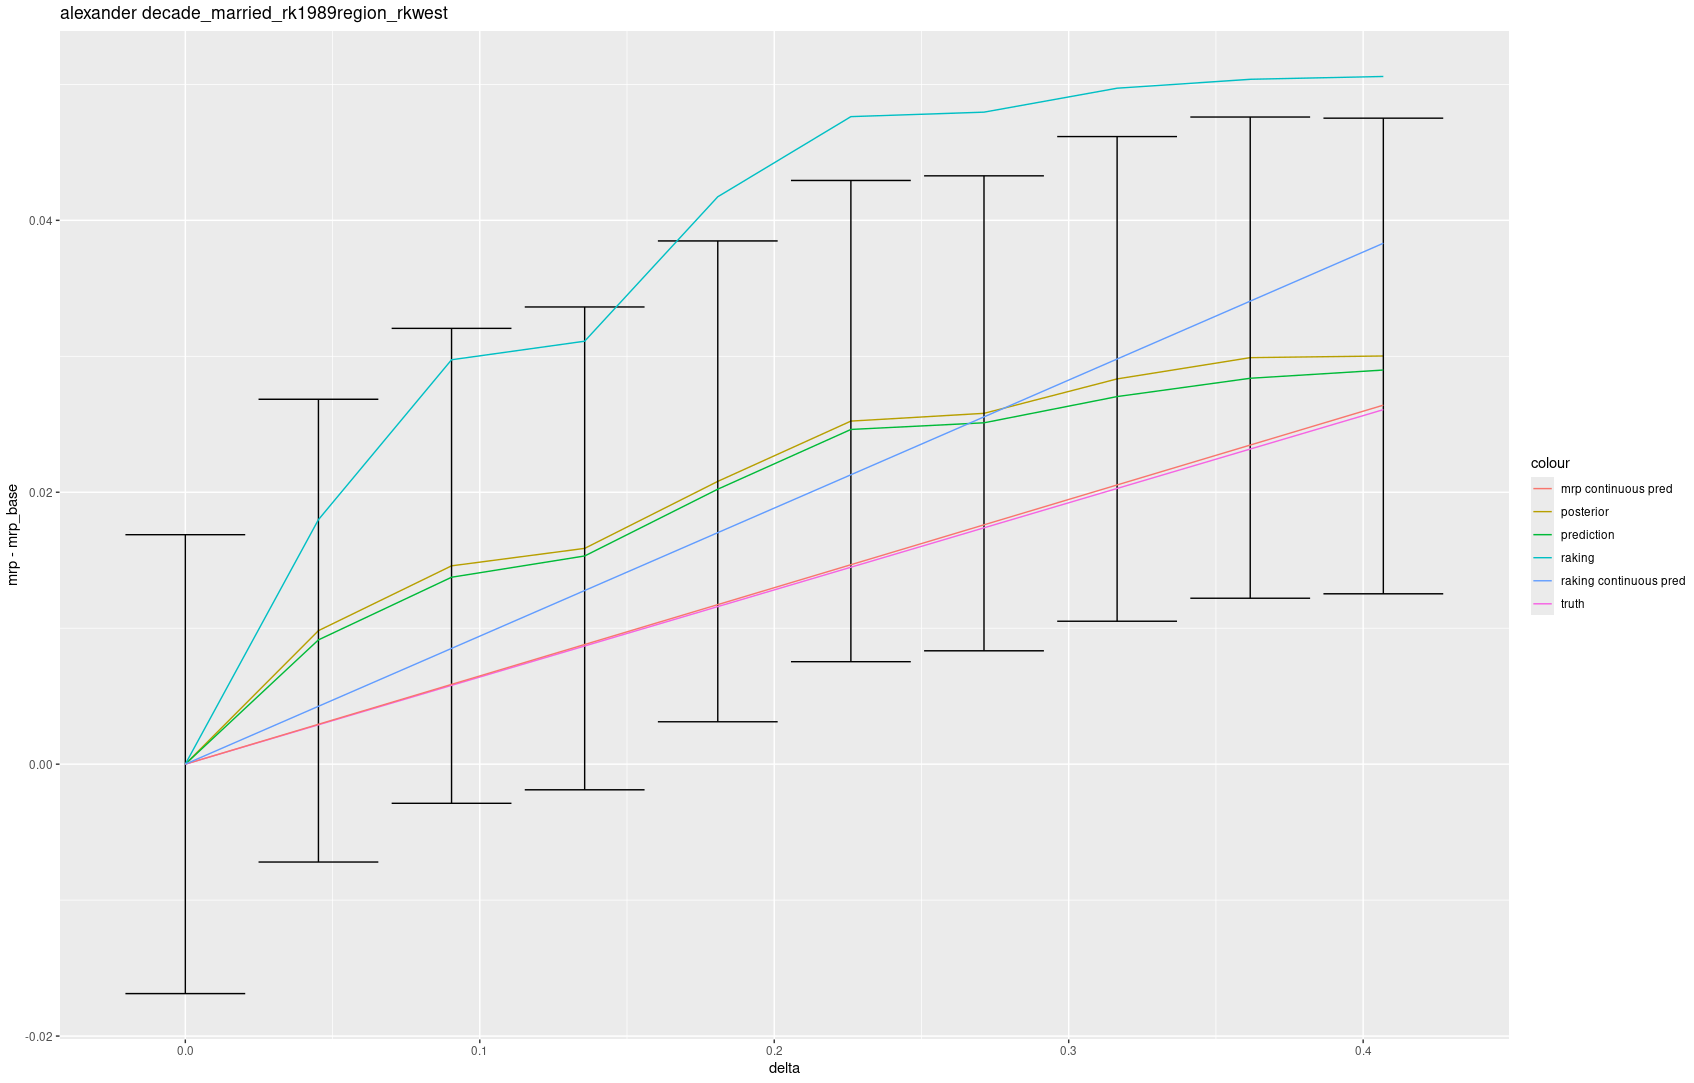
\includegraphics[height=0.9\textheight]{static_figures/mrpaw.png}
\end{frame}



\begin{frame}{Future work and generalizations}
%
\begin{itemize}
    \item Instance of a very general class of local consistency checks that generalize
          classical regression checks (work with Sequoia)
    \item Versions for GLMMs (work with Vladimir)
    \item Going beyond classical Bayesian sensitivity (work with Lucas)
\end{itemize}
%
\end{frame}


%%%%%%%%%%%%%%%%%%%%%%%%%%%%%%%%%%%%%%%%%%%%%%%%%%%%%%%%%%%%%%%%%%%%%%%%%%%
%%%%%%%%%%%%%%%%%%%%%%%%%%%%%%%%%%%%%%%%%%%%%%%%%%%%%%%%%%%%%%%%%%%%%%%%%%%
%%%%%%%%%%%%%%%%%%%%%%%%%%%%%%%%%%%%%%%%%%%%%%%%%%%%%%%%%%%%%%%%%%%%%%%%%%%


\begin{frame}{References}

\footnotesize

\bibliographystyle{plainnat}
% Hide the references header
% https://tex.stackexchange.com/questions/22645/hiding-the-title-of-the-bibliography/370784
\begingroup
\renewcommand{\section}[2]{}%
\bibliography{references}
\endgroup

\end{frame}


\end{document}
